\documentclass[a4paper,11pt]{report}
\usepackage{geometry}\geometry{a4paper,top=3cm,bottom=3cm,left=2cm,right=2cm,heightrounded,bindingoffset=0mm}
%ocio al bindingoffset!
\usepackage[T1]{fontenc}
\usepackage[utf8]{inputenc}
\usepackage[italian]{babel}
\usepackage{amsmath,amsfonts,amssymb,braket}
\usepackage{graphicx}
%\usepackage{subfig} %sub-figures
\usepackage{epsfig}
\usepackage{titlesec} % per formato custom dei titoli dei capitoli
\usepackage{csvsimple}
\usepackage[output-decimal-marker={,}]{siunitx}
\usepackage{lipsum}

%Some usefull commands
\usepackage{xspace}% per lo spazio intelligente
\newcommand{\e}{\`E\xspace}  %E'
\renewcommand{\si}{\SI}
\begin{document}
\pagestyle{plain}
\thispagestyle{empty}
\begin{center}
  \begin{figure}[H]
    \centerline{
\psfig{file=Img/logo_unitn_black_center.eps,
                        width=0.8\textwidth,trim = 0 0.9cm 0 0.5cm}}
  \end{figure}
\line(1,0){450}

  \large\textsc{Dipartimento di Ingegneria Civile, Ambientale e Meccanica\\}
  \large{Corso di Laurea in Ingegneria Civile
  }

  \vspace{3.7 cm} 
  %\Large\textsc{Elaborato finale\\} 
  %\vspace{1 cm} 
  \Huge\textsc{relazione di topografia\\}
  
  \vspace{0.2 cm}
  \Large{\it{Descrizione e rielaborzione di esempi e rilievi eseguiti}}


  \vspace{4 cm} 
  \begin{tabular*}{\textwidth}{ l @{\extracolsep{\fill}} r }
  \Large\textsc{Docente} & \Large\textsc{Studenti}\\
  \Large{Battista Benciolini}& \Large{Nicola Meoli 186100}\\
  \Large{Alfonso Vitti}& \\
  \Large{Paolo Zatelli}& \\
        
  \end{tabular*}

  \vspace{3.1cm} 
    \line(1,0){450}
    
  \Large{Anno accademico 2018/19}
  
\end{center}
\tableofcontents
% redefinizione del formato del titolo del capitolo
      % da formato
      %   Capitolo X
      %   Titolo capitolo
      % a formato
      %   X   Titolo capitolo 
	\titleformat{\chapter}
        {\normalfont\Huge\bfseries}{\thechapter}{1em}{}
	\titlespacing*{\chapter}{0pt}{0.59in}{0.02in}
	\titlespacing*{\section}{0pt}{0.20in}{0.02in}
	\titlespacing*{\subsection}{0pt}{0.10in}{0.02in}
%---        
\chapter{Descrizione del lavoro svolto}
\setcounter{page}{1}
Le esercitazioni strumentali si sono svolte in tre diverse giornate presso il  parco della facoltà di Mesiano, in ciascuna delle quali si è affrontato un diverso tipo di rilievo.
In ogni giornata si sono dapprima viste le modalità di utilizzo degli strumenti e il loro corretto stazionamento.
Al quale è poi seguito un piccolo lavoro di rilievo di alcuni punti concordati e con le opportune convenzioni.

Nelle tre diverse giornate si è affrontato, rispettivamente, l'utilizzo del livello, del GNSS e della stazione totale. 
Si parlerà ora con maggior dettaglio delle tre tipologie, e nei capitoli successivi si potranno vedere le rielaborazioni svolte con i dati raccolti.
\section{Livello}
L'esercitazione mediante livello si è svolta il giorno 12 marzo 2019 nella zona adiacente al parcheggio multi-piano di Mesiano.
Dopo una rapida spiegazione del funzionamento degli strumenti e della loro corretta messa in stazione, si è svolta l'attività di rilievo. 

L'obiettivo del lavoro era quello di effettuare delle misure di dislivello tra quattro diversi punti e di chiudere l'ultima livellazione con la prima. 
Si è perciò iniziato con la messa in stazione dello strumento, consistente nel far sì che l'asse primario fosse verticale e passante per il punto a terra grazie all'ausilio di una livella sferica e del compensatore integrato nel livello.  

Nelle diverse letture alla stadia si è utilizzato anche il micrometro per poter leggere fino alla quarta cifra decimale.
Come modalità operative nei diversi punti si sono utilizzate sia livellazioni dal mezzo -- ovvero quelle in cui il livello sta a metà tra due stadie -- sia livellazioni reciproche, con il livello prima vicino ad una stadia e poi all'altra.
La diversa lettura di queste la si nota nei libretti di campagna riportati nel  capitolo \ref{cap:cap2} e nei calcoli collegati. 

Per ogni punto si sono eseguite più coppie di letture (avanti e indietro), ognuna delle quali fatta da un operatore diverso. Così come la tenuta \emph{in verticale} delle stadie è avvenuta da persone diverse a turno. 
Sì è così venuta a creare una serie di misure ripetute, le quali verranno poi analizzate nei capitoli successivi.
\section{GNSS}
Il giorno 19 marzo 2019 si è svolta l'esercitazione tramite il sistema GNSS. \e avvenuta nel parco di Mesiano, prima nella zona adiacente al laboratorio di Meccanica dei Fluidi, per poi estendersi in altri punti segnati a terra tramite chiodo attorno all'edificio principale.

\e stata fatta prima una spiegazione con una carrellata nei menù dello strumento di tute le possibili modalità di rilievo fattibili, per poi concentrarsi nella modalità \emph{Real Time Kinematic} (RTK) con la quale sono stati raccolti i dati.
La modalità RTK è stata eseguita appoggiandosi al servizio offerto dalla Provincia Autonoma di Trento \emph{TPOS} grazie il quale è possibile utilizzare come ricevitore una stazione fissa con noti a priori la posizione e i disturbi atmosferici, così da elaborare in tempo reale la posizione del secondo ricevitore.

Il rilievo è consistito nella misura di posizione dei punti prefissati e nell'accertarsi che ci fossero abbastanza satelliti in vista da far risultare un'accuratezza dell'ordine del centimetro. 
Misure che sono state poi rielaborate eseguendo una rototraslazione nel capitolo \ref{cap:cap3}.
\section{Stazione totale}
Il giorno 26 marzo 2019 è avvenuta l'ultima esercitazione, questa volta con l'ausilio di una stazione totale e del prisma per la misura delle distanze. 
Sono stati usati inoltre appositi supporti per il mantenimento in verticale del prisma.
La zona interessata è quella tra il laboratorio e il parcheggio multi-piano di Mesiano. 

L'obiettivo era quello di eseguire letture zenitali e azimutali di tre punti concordati a formare un triangolo e di misurarne la distanza tra essi tramite il distanziometro. 
La messa in stazione è avvenuta in coincidenza con i tre punti e da ognuna sono stati collimati i due punti rimanenti. 
Letture che anche in questo caso sono state eseguite a rotazione tra i vari operatori.
\chapter{Livellazione}\label{cap:cap2}
%LIBRETTO: comando per importare i libretti dal csv
\newcommand{\libretto}[3]{
\begin{table}[htb]\footnotesize
\caption{#1}
\label{#2}
\centering
\csvreader[centered tabular=c@{}SSSSSSSS,
	table head=\toprule &$\mathbf{L_{dx}}$ & $\mathbf{L_{sx}}$ & $\mathbf{L_{dx}}$ %
	& $\mathbf{L_{sx}}$ & $\mathbf{L_{dx}}$ & $\mathbf{L_{sx}}$ & $\mathbf{L_{dx}}$ & $\mathbf{L_{sx}}$ \\\midrule,
	table foot = \bottomrule]%
	{#3}{}%
	{&\csvcoli & \csvcolii & \csvcoliii & %
	\csvcoliv & \csvcolv & \csvcolvi & %
	\csvcolvii & \csvcolviii}
\end{table}}
%ELABORAZIONE: comando per importare le rielaborazione dei libretti
%1: caption, 2: label, 3: percorso file
\newcommand{\elaborazione}[3]{
\begin{table}[htb]\footnotesize
\caption{#1}
\label{#2}
\centering
\csvreader[centered tabular=c@{}rSSSSSSSS,
	no head, %nel csv non c'è la riga iniziale come nei libretti
	table head=\toprule &&$\mathbf{1}$ & $\mathbf{2}$ & $\mathbf{3}$ %
	& $\mathbf{4}$ & $\mathbf{5}$ & $\mathbf{6}$ & $\mathbf{7}$ & $\mathbf{8}$ \\\midrule,
	table foot = \bottomrule]%
	{#3}{}%
	{&\textbf{\csvcolix} & \csvcoli & \csvcolii & \csvcoliii & %
	\csvcoliv & \csvcolv & \csvcolvi & %
	\csvcolvii & \csvcolviii}
\end{table}}
%----------------------------------------
Si riporta innanzitutto il libretto di campagna nella tabella  \ref{tab:libretto1}.
\section{Primo libretto}
\libretto{Libretto di campagna del gruppo 3}{tab:libretto1}{documents/livLibretto1.csv}
\elaborazione{Elaborazione del libretto di campagna assegnando peso 1 a tutte le misure}{tab:libretto1rielaborato}{documents/livLibretto1rielaborato.csv}
\elaborazione{Rielaborazione dopo aver modificato i pesi delle misure}{tab:libretto1rielaboratoaggiustato}{documents/livLibretto1rielaboratoaggiustato.csv}
%
\clearpage %mette tutti i float fin qua definiti
\section{Secondo libretto}
\libretto{Libretto di campagna del gruppo 3}{tab:libretto2}{documents/livLibretto2.csv}
\elaborazione{Elaborazione del libretto di campagna assegnando peso 1 a tutte le misure}{tab:libretto2rielaborato}{documents/livLibretto2rielaborato.csv}
\elaborazione{Rielaborazione dopo aver modificato i pesi delle misure}{tab:libretto2rielaboratoaggiustato}{documents/livLibretto2rielaboratoaggiustato.csv}



\chapter{Rototraslazione e variazione di scala}\label{cap:cap3}
Una generica rototraslazione con annessa variazione di unità di misura tra due diversi sistemi di riferimento si effettua mediante:
\begin{equation}
	\label{eq:roto}
	\underline{y}=\mu \mathbf{R} \underline{x}+\underline{t}
\end{equation}
in cui se le coordinate nei due sistemi di riferimento sono note e se si è nel caso bidimensionale, si possono calcolare i parametri $\mu$,$\alpha$,$t_{(1)}$ e $t_{(2)}$.
Per farlo è opportuno linearizzare i parametri della matrice di rotazione $\mathbf{R}$ sostituendo ai suoi elementi i nuovi parametri $a=\mu\cos\alpha$ e $b=\mu\sin\alpha$:
\[
\mathbf{R}=
\begin{bmatrix}
\cos\alpha & -\sin\alpha \\ 
\sin\alpha & \cos\alpha
\end{bmatrix} 
\quad \Longrightarrow \quad
\mu \mathbf{R} = 
\begin{bmatrix}
a & -b \\ 
b & a
\end{bmatrix} 
\]
\e necessario poi minimizzare la funzione $\Phi$ definita come la somma del vettore degli scarti vettoriali trasposto per lo stesso non trasposto.
\e così possibile così stimare i parametri $\hat{a}$ e $\hat{b}$ partendo dalle coordinate iniziali dei punti $k$ $\underline{x_k}$ e $\underline{y_k}$ nei diversi sistemi.
Si calcolano dapprima le media del baricentro:
\begin{align}
\underline{x_B} &= \frac{1}{N}\sum_{k=1}^{N}\underline{x_k}\\
\underline{y_B} &= \frac{1}{N}\sum_{k=1}^{N}\underline{y_k}
\end{align}
per poi calcolare le coordinate baricentriche come differenza tra le coordinate iniziali e la media del baricentro:
\begin{align}
\overline{\underline{x_k}} &= \underline{x_k} - \underline{x_B}\\
\overline{\underline{y_k}} &= \underline{y_k} - \underline{y_B}
\end{align}
Ridefinendo il vettore $\underline{t}$ come $\underline{t_{0}}=\underline{t}-\underline{w}_{B}+\lambda \mathbf{R} \underline{u}_{B}$ è possibile riportarsi all'equazione \ref{eq:roto} in cui però compaiono le coordinate baricentriche.
\begin{equation}
\underline{y_{k}}=
\begin{bmatrix}
	{a} & {-b} \\ 
	{b} & {a}
\end{bmatrix} 
\overline{x_{k}}+\underline{t_{0}}
\end{equation}
che in forma espansa diventa:
\begin{equation}
	\begin{bmatrix}
		\underline{y}_{k(1)} \\ 
		\underline{y}_{k(2)}
	\end{bmatrix} 
	=
	\begin{bmatrix}
		{a} & {-b} \\ 
		{b} & {a}
	\end{bmatrix}
	\begin{bmatrix}
		\underline{x}_{k(1)} \\ 
		\underline{x}_{k(2)}
	\end{bmatrix}
	+
	\begin{bmatrix}
		\underline{t}_{(1)} \\ 
		\underline{t}_{(2)}
	\end{bmatrix}
\end{equation}
Chiamando il vettore dei termini noti con $\underline{\eta}$, quello dei termini incogniti con $\underline{\xi}$ e con $\mathbf{A}$ la matrice dei coefficienti, si ha:
\begin{equation}
	\underline{\eta}=\mathbf{A} \underline{\xi}
\end{equation}
Si tratta di un sistema facilmente risolvibile se si considerano le coordinate $x$ note senza errori e le coordinate $y$ con pari varianza e non correlate tra loro. 
\begin{equation}
	\hat{\underline{\xi}}=	
	\left(\mathbf{A}^T \mathbf{A}\right)^{-1}
	\left(\mathbf{A}^T \underline{\eta}\right)
\end{equation}
Permette così di trovare i parametri $d$, $p$, $q$, $a$ e $b$:
\begin{align} d &=\sum_{k=1}^{N}\left(\overline{x}_{k(1)}^{2}+\overline{x}_{k(2)}^{2}\right) \\ 
p &=\sum_{k=1}^{N}\left(\overline{x}_{k(1)} \overline{y}_{k(1)}+\overline{x}_{k(2)} \overline{y}_{k(2)}\right) \\ 
q &=\sum_{k=1}^{N}\left(\overline{x}_{k(1)} \overline{y}_{k(2)}-\overline{x}_{k(2)} \overline{y}_{k(1)}\right) \\
\hat{a} &= \frac{p}{d} \\
\hat{b} &= \frac{q}{d}
\end{align}
Grazie ai quali è possibile calcolare le stime $\hat{\mu}$, $\hat{\alpha}$ e il vettore degli scarti $\underline{v}$.
Quest'ultimo ottenuto minimizzando la funzione:
\begin{equation}
	\Phi = \sum_k \underline{v}^T\underline{v}_k
\end{equation}
\begin{align}
	\hat{\mu} &= \sqrt{\hat{a}^2 + \hat{b}^2}\\
	\hat{\alpha} &= \arctan\frac{\hat{b}}{\hat{a}}\\
	\underline{v_k} &= 
	\overline{\underline{y_{k}}}-
\begin{bmatrix}
	\hat{a} & -\hat{b} \\ 
	\hat{b} & \hat{a}
\end{bmatrix} 
\overline{x_{k}}
\end{align}
\section{Esempio applicativo}
Come esempio si applica il metodo appena visto a questi dati iniziali:


Lo stesso esempio è stato rifatto all'interno di un foglio elettronico ottenendo ovviamente gli stessi risultati.
\begin{figure}[H]
\centering
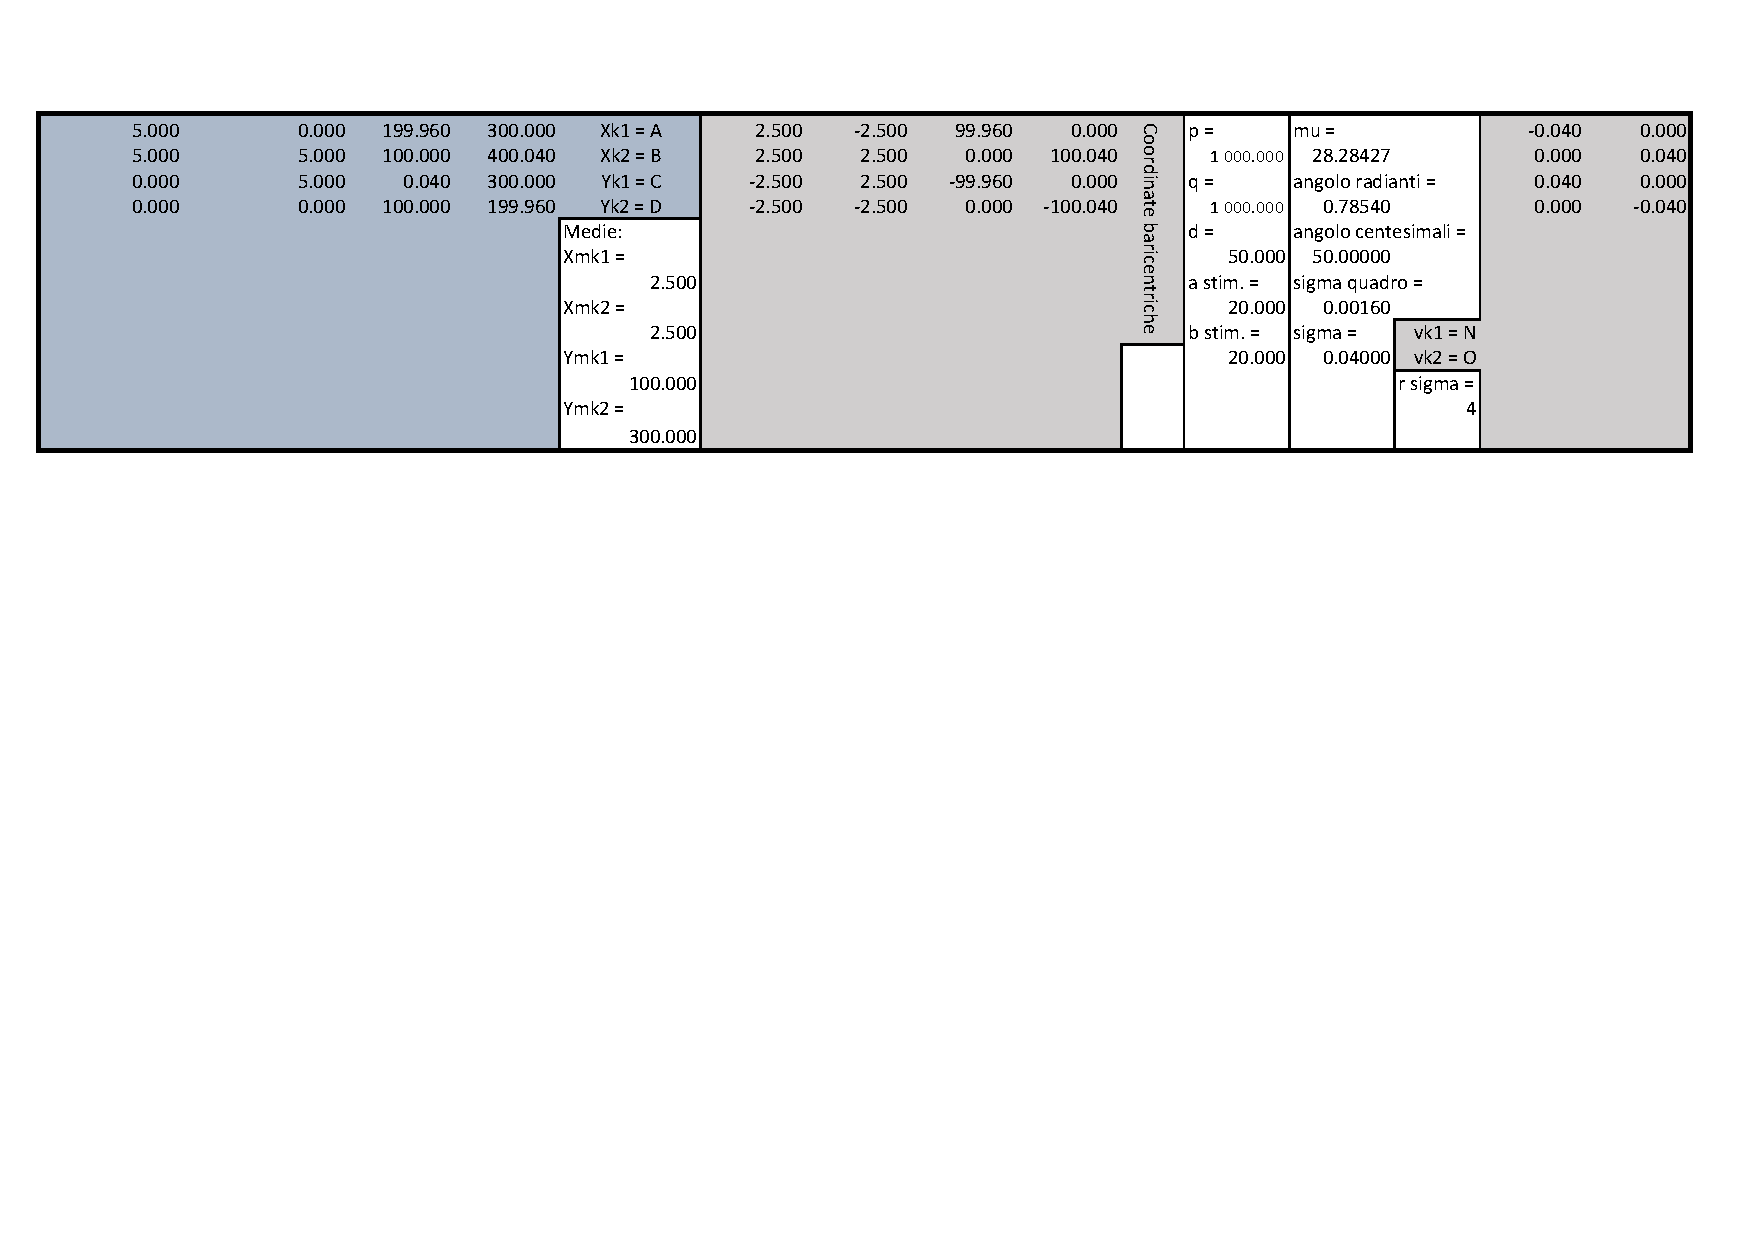
\includegraphics[width=16cm]{documents/rototraslazioneEsempio.pdf}
\end{figure}
\section{Rototraslazione ad un rilievo reale}
Il metodo visto ed eseguito in foglio di calcolo lo si applica ora ad un rilievo con i seguenti dati iniziali:
BLABLABLA
\begin{figure}[H]
\centering
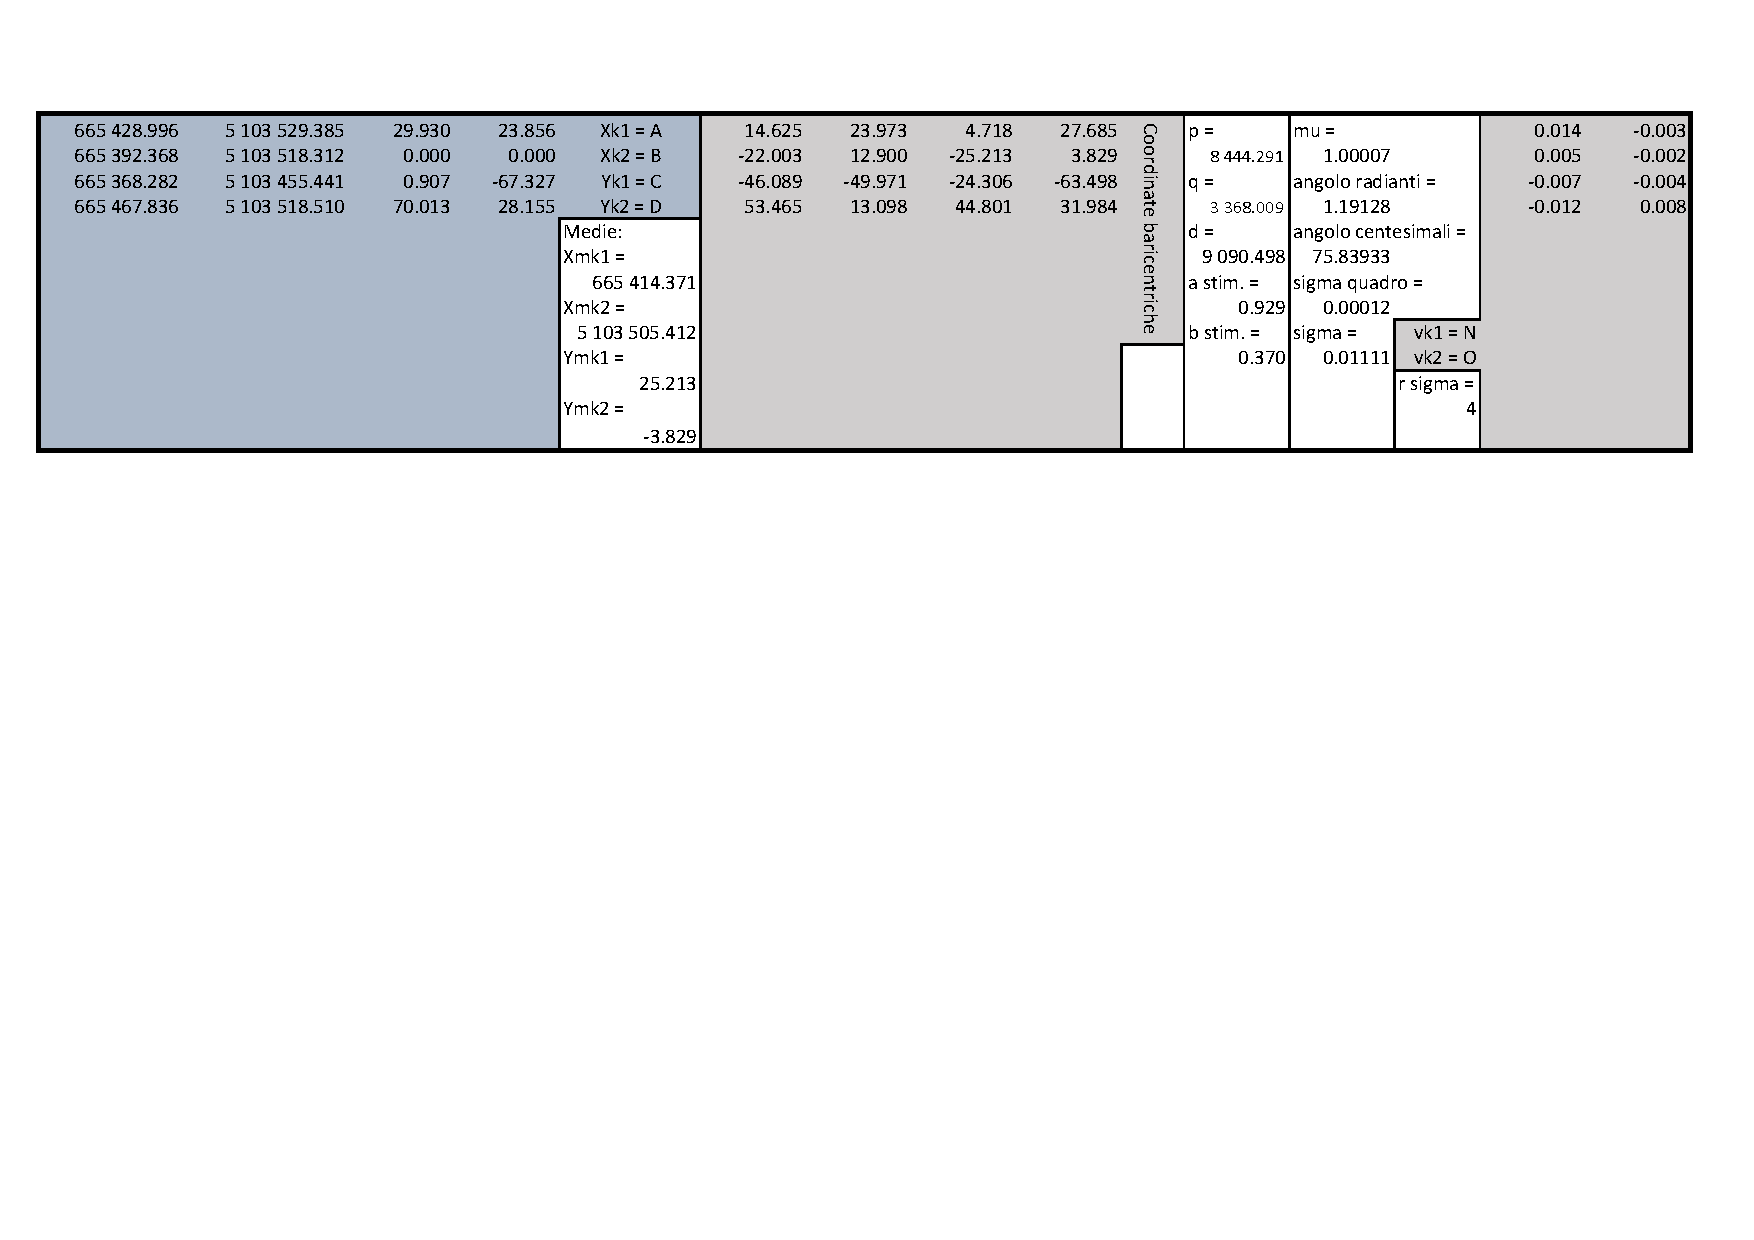
\includegraphics[width=16cm]{documents/rototraslazioneRilievo.pdf}
\end{figure}
	
%\vec: freccia (fisica)
%\boldsymbol: corsivo matematico
%\mathbf: tondo nero

%!TEX root = ../Topografia_Relazione_MeoliNicola.tex
\chapter{Compatibilità e compensazione}\label{cap:cap4}
Con i dati raccolti durante le esercitazioni con stazione totale svolte dai vari gruppi, si è proceduto ad eseguire dei controlli di compatibilità tra alcune grandezze plano-altimetriche.
In particolare si sono calcolati i valori mediati delle misure ripetute, controllate le chiusure planimetriche degli angoli e delle distanze e le chiusure altimetriche dei dislivelli.
Si è perciò controllato che la somma degli angoli interni formasse un angolo piatto. 
Che i lati opposti del triangoli rispettassero il teorema dei Carnot, confrontando lato calcolato con il lato misurato. 
E infine che la somma dei dislivelli risultasse zero.

Nel caso di misure palesemente con errori grossolani "a vista" le si è eliminate.
Con le restanti, invece, si è eseguita una compensazione con il programma Calge, confrontando le varianze ed eliminando le misure inadeguate, al fine di ottenere le coordinate dei punti del triangolo. 
\begin{align}
	\sum \alpha^{int.} &\cong \si{200}{^g} \label{eq:somma200}\\
	c^{mis.} &\cong c^{calc.} = \sqrt{a^2 + b^2 - 2ab\cos(\gamma)} \label{eq:carnot}\\
	\sum \Delta_i &\cong 0 \label{eq:somma0}
\end{align}

Si riporta di seguito la procedura appena descritta per i dati raccolti dal gruppo 1 e dal gruppo 3 delle esercitazioni. Il disegno del rilievo è riportato in figura \ref{fig:Triangolo} del capitolo \ref{cap:cap1}. Si riporterà poi un esempio di compensazione eseguito conoscendo le distanze.

Obiettivo della compensazione è quello di riuscire ad ottenere risultati adeguati togliendo le misure ripetute che si rilevano troppo discostanti dalle medie, senza però ottenere valori di $\sigma_0$ inferiori all'unità, in quanto poi i risultati finali perderebbero di significato. 

L'ordine di lettura degli input esposti qui di seguito consistono per le prime due comppensazioni in:
\begin{lstlisting}
AAAA , I , X , Y , Z  
......
AAAA , BBBB , J , dist , direz_azim , angolo_zenitale , H_strum_BBBB , H_strum_AAAA
\end{lstlisting}
mentre per l'ultima compensazione in:
\begin{lstlisting}
AAAA , BBBB , K , misura
\end{lstlisting}
Dove con $I$ si intende il parametro per indicare i gradi di libertà di quel punto, con $J$ l'indice per indicare se è accettata o meno quella misura ($0 = $ OK) e con $K$ la tipologia di misura: distanza nel nostro caso.
\section{Compensazione del rilievo del gruppo 1}
Per eseguire i controlli di compatibilità descritti dalle \eqref{eq:somma200}, \eqref{eq:carnot} e \eqref{eq:somma0} è stato necessario adattare i dati di partenza riportati nella tabella \ref{tab:DatiInit1} rappresentante il libretto di campagna già precedentemente adattato, eliminando gli errori grossolani e ordinando le misure.
%Tabella dati iniziali gruppo1
\begin{table}[htb]\footnotesize
\caption{Dati di partenza ottenuti dal libretto di campagna del gruppo 1 e da cui si sono fatti i controlli di compatibilità}
\label{tab:DatiInit1}
\centering
\csvreader[centered tabular=c@{}ccSSSSS,
	no head, %nel csv non c'è la riga iniziale come nei libretti
	table head=\toprule & {P. stazione} & {P. collimato} & {Dist.} & {Dir. azimutale} %
	& {Angolo zenitale} & {Alt. prisma} & {Alt. teodolite}  \\\midrule,
	table foot = \bottomrule]%
	{documents/TriangoloCivile2019gruppo1.csv}{}%
	{& \csvcoli & \csvcolii & \csvcoliv & \csvcolv & \csvcolvi &	\csvcolvii &\csvcolviii}
\end{table}

Per prima cosa si sono calcolati gli angoli azimutali eseguendo la differenza delle letture misurate o mediate - nel caso fosse misure ripeture - ottenendo:
\begin{align*}
\widehat{213} = \si{71.38490}{^g}\\
\widehat{123} = \si{68.64625}{^g}\\
\widehat{132} = \si{59.96810}{^g}\\
\end{align*}
e sommandoli si ottiene \si{0.00075}{^g} che rappresenta un errore di chiusura planimetrica particolarmente accettabile. Soprattutto se confrontato con quello degli altri gruppi.

Per quanto riguarda il controllo dei lati opposti è stato necessario calcolare prima le distanze orizzontali utilizzando l'angolo zenitale
\[
	d_{oriz.} = d_{incl.} \, \sin{z}
\]
per poi calcolare i lati con la formula di Carnot e confrontare misurato con calcolato, ottenendo differenze di non più un centimetro:
\begin{center}
\begin{tabular}%
		{c%
		S[table-format=2.3]%
		S[table-format=2.3]}
\toprule
& {Misurato} & {Calcolato}  \\ \midrule
$\overline{12}$ & 32.830 & 32.831\\
$\overline{23}$ & 36.564 & 36.573 \\
$\overline{31}$ & 35.771 & 35.770 \\
\bottomrule
\end{tabular}
\end{center}

Nella verifica altimetrica si sono calcolati i dislivelli delle varie misure elaborando i dati con la classica formula 
\[
	d_{incl.} \cos{z} + H_{teod.} - H_{prisma}
\]
e tenendo conto del loro verso. Sommandoli si è ottenuto un errore di chiusura di \si{-0.014}{m}.

\e stata poi affrontata la compensazione vera e propria eseguita con il programma Calge.
Per ottenere le coordinate di partenza da cui far partire il processo di iterazione di Calge, si è assegnata al punto $3000$ l'origine degli assi e si è posto l'orientamento dell'asse $x$ verso il punto $1000$ con ascissa assegnata pari a $36$. Per le quote si è tenuto conto di un dislivello medio di 4 metri.
All'inizio si sono utilizzate tutte le misure effettuate, che possono essere lette nell'input del programma qui di seguito. 
\begin{lstlisting}
1000, 4, 	36, 		0, 	4
2000, 0 , 	20,	 	30,	4
3000, 1, 	0, 		0, 	0
$$$$, 0,0,0,0
1000,2000,0,32.859,     392.93545,  102.3237,   1.522,  1.516
1000,3000,0,36.28,      321.55055,  110.56335,  1.600,  1.516
2000,1000,0,32.856,     189.2002,   97.44795,   1.600,  1.522
2000,1000,0,32.856,     189.2017,   97.4526,    1.600,  1.522
2000,3000,0,36.896,     257.8463,   108.5599,   1.467,  1.522
2000,3000,0,36.896, 	257.8481,   108.554,    1.467,  1.522
3000,1000,0,36.315, 	224.8441,   88.96775,   1.600,  1.467
3000,2000,0,36.896, 	164.876,    91.4474,    1.522,  1.467
xxxx,xxxx,0,0,0,0,0,0
GRUPPO UNO
\end{lstlisting}
Il quale porta ad un risultato che presenta un residuo troppo elevato nell'angolo zenitale della misura a riga 6.
Si è perciò eliminata tale misura portando ad avere un nuovo residuo nella riga 5 e che ha un $\sigma_0^2$ pari a \si{1.7233}{}.
Si è eliminata anche tale riga, rifacendo il calcolo. 
\e però stato scartato questo nuovo input perché $\sigma_0^2$ è diventata pari a \si{0.1568}{}.

Si è quindi tenuto come risultato finale quello in cui si è eliminata soltanto riga 6 e che porta alle seguenti coordinate dei punti:
%Coordinate gruppo 1
\begin{center}
\begin{tabular}%
		{c%
		S[table-format=2.6]%
		S[table-format=2.6]%
		S[table-format=2.6]}
\toprule
& {$\mathbf{x}$} & {$\mathbf{y}$} & {$\mathbf{z}$}   \\ \midrule
$\mathbf{1000}$ & 35.771665  &  0.000000 &  6.120490 \\
$\mathbf{2000}$ & 21.505886  & 29.570282 &  4.890624 \\
$\mathbf{3000}$ &  0.000000  &  0.000000  & 0.000000 \\
\bottomrule
\end{tabular}
\end{center}
%
\section{Compensazione del rilievo del gruppo 3}
%Tabella dati iniziali gruppo 3
\begin{table}[htb]\footnotesize
\caption{Dati di partenza ottenuti dal libretto di campagna del gruppo 3 e da cui si sono fatti i controlli di compatibilità}
\label{tab:DatiInit3}
\centering
\csvreader[centered tabular=c@{}ccSSSSS,
	no head, %nel csv non c'è la riga iniziale come nei libretti
	table head=\toprule & {P. stazione} & {P. collimato} & {Dist.} & {Dir. azimutale} %
	& {Angolo zenitale} & {Alt. prisma} & {Alt. teodolite}  \\\midrule,
	table foot = \bottomrule]%
	{documents/TriangoloCivile2019gruppo3.csv}{}%
	{& \csvcoli & \csvcolii & \csvcoliv & \csvcolv & \csvcolvi &	\csvcolvii &\csvcolviii}
\end{table}
Lo stesso procedimento è stato eseguito per il gruppo 3 con i dati riportati in tabella \ref{tab:DatiInit3} a pagina \pageref{tab:DatiInit3}. Si riporta sommariamente gli errori di chiusura e le coordinate dei punti.
In generale il rilievo del gruppo 3 presenta degli errori che sono diffusi un po' a tutte le misure e pertanto non sempre si è riusciti a sistemarli eliminando le misure contenenti errori grossolani.
\begin{align*}
\widehat{213} &= \si{70.79045}{^g}\\
\widehat{123} &= \si{68.04815}{^g}\\
\widehat{132} &= \si{61.11460}{^g}\\
\text{Errore}_{plan.} &= \si{00.04680}{^g} 
\end{align*}

\begin{center}
\begin{tabular}%
		{c%
		S[table-format=2.3]%
		S[table-format=2.3]}
\toprule
& {Misurato} & {Calcolato}  \\ \midrule
$\overline{12}$ & 33.213 & 33.215\\
$\overline{23}$ & 36.363 & 36.354 \\
$\overline{31}$ & 35.549 & 35.544 \\
\bottomrule
\end{tabular}
\end{center}
e un errore di chiusura verticale di $\si{-0.012}{m}$.

Per quanto riguarda la compensazione eseguita con Calge, invece.
\begin{lstlisting}
1000, 4,	36,	0,  	4
2000, 0 ,	20, 	30, 	4
3000, 1, 	0, 	0,   	0
$$$$, 0,0,0,0
1000,2000,0,33.235,	194.6851,	102.32575,	1.408,	1.399
1000,3000,0,36.047,	123.89465,	110.4399,	1.600,	1.399
2000,1000,0,33.243,	26.779,		97.2715,	1.602,	1.408
2000,1000,0,33.244,	26.78865,	97.27255,	1.602,	1.408
2000,3000,0,36.684,	94.83175,	108.4262,	1.441,	1.408
2000,3000,0,36.684,	94.8322,	108.42515,	1.441,	1.408
3000,1000,0,36.097,	330.8344,	88.8924,	1.602,	1.441
3000,2000,0,36.684,	269.7198,	91.57075,	1.408,	1.441
xxxx,xxxx,0,0,0,0,0,0
GRUPPO TRE
\end{lstlisting}
Utilizzando il qui sopra esposto libretto si ottiene un residuo elevato nella seconda misura. 
Si è perciò eliminata la riga 6 portando ad un $\sigma_0^2$ pari a \si{2.1511}{}.
Facendo varie prove si è notato che eliminando altre righe comportava ad avere $\sigma_0^2$ troppo bassi, pertanto si è mantenuto il risultato ottenuto avendo tolto solo la seconda misura (riga 6 dell'input).

In questo caso si sono ottenuti valori di varianze più elevate rispetto al gruppo 1 e soprattutto con errori non attribuibili ad una specifica misura.
Tale considerazione la si può vedere confrontando i valori delle singole coordinate. 

Si ottengono pertanto le seguenti coordinate dei punti:
%Coordinate gruppo 1
\begin{center}
\begin{tabular}%
		{c%
		S[table-format=2.6]%
		S[table-format=2.6]%
		S[table-format=2.6]}
\toprule
& {$\mathbf{x}$} & {$\mathbf{y}$} & {$\mathbf{z}$}   \\ \midrule
$\mathbf{1000}$ & 35.544380 & 0.000000 & 6.106777 \\
$\mathbf{2000}$ & 20.855675 &29.788713 & 4.876273 \\
$\mathbf{3000}$ &  0.000000 & 0.000000 & 0.000000 \\
\bottomrule
\end{tabular}
\end{center}

%

\section{Esempio in aula}
In questo caso si è affrontato un problema nel quale si era a conoscenza delle distanze misurate e le si doveva confrontare con i lati calcolati partendo dalle coordinate dei punti. 
\begin{lstlisting}
1000, 1, 	1.2, 		0,0
2000, 1 , 	0,	 	0,0
3000, 0, 	0, 		0,0
$$$$, 0,	0,	0,0
1000, 3000,	0,	1.0220290
2000,3000,	0,	1.0102192
xxxx,xxxx,	0,	0
TRIANGOLO
\end{lstlisting}

\chapter{Rototraslazione e variazione di scala}
bla bla bla
%-----bibliografy
%\nocite{name} %uncomment with the right name
%\bibliographystyle{plain}
%\bibliography{biblio}

\end{document}